\documentclass[11pt]{article}
\usepackage{cornell-notes}
\usepackage{mathtools}
\usepackage{needspace}
\usepackage{ragged2e}
\usepackage{adjustbox}
\usepackage{tikz}
\usetikzlibrary{arrows.meta,positioning}
\tcbuselibrary{most}
\geometry{letterpaper,margin=0.72in,headheight=15pt}
\setCornellCollection{Calculus Cornell Notes}
\setCornellUnitType{Chapter}
\setCornellUnitNumber{13}
\setCornellUnitTitle{Functions of Several Variables}

\definecolor{Ink}{HTML}{17324D}
\definecolor{Teal}{HTML}{147D78}
\definecolor{Sky}{HTML}{DDEEF1}
\definecolor{Cue}{HTML}{EEF2F5}
\definecolor{Warm}{HTML}{FFF3D6}
\definecolor{Alert}{HTML}{9D3C32}
\definecolor{Green}{HTML}{276749}
\definecolor{Rule}{HTML}{AAB8C2}
\hypersetup{colorlinks=true,linkcolor=Ink,urlcolor=Teal,pdfborder={0 0 0}}
\setlength{\parindent}{0pt}
\setlength{\parskip}{4pt}
\setlist{nosep,leftmargin=*}
\titleformat{\section}{\Large\bfseries\color{Ink}}{}{0pt}{}[\color{Teal}\titlerule]
\titleformat{\subsection}{\large\bfseries\color{Teal}}{}{0pt}{}
\pagestyle{fancy}
\fancyhf{}
\fancyhead[L]{\small\color{Ink}\textsc{Cornell Notes}}
\fancyhead[R]{\small\color{Teal}\nouppercase{\leftmark}}
\fancyfoot[L]{\footnotesize\color{Ink}Active recall $\bullet$ Worked reasoning $\bullet$ Verification}
\fancyfoot[R]{\footnotesize\color{Ink}\thepage\ of \pageref*{LastPage}}
\renewcommand{\headrulewidth}{0.5pt}
\renewcommand{\footrulewidth}{0.4pt}
\newcolumntype{Y}{>{\RaggedRight\arraybackslash}X}
\newtcolorbox{orientationbox}{enhanced,breakable,colback=Sky,colframe=Teal,boxrule=0.7pt,arc=2mm,title=Chapter orientation,fonttitle=\bfseries}
\newtcolorbox{sectionsummarybox}{enhanced,breakable,colback=white,colframe=Teal,boxrule=0.6pt,arc=1.5mm,left=2mm,right=2mm,top=1mm,bottom=1mm,title=Section synthesis,fonttitle=\bfseries\color{Teal}}
\newtcolorbox{warningbox}{enhanced,breakable,colback=Warm,colframe=Alert,boxrule=0.7pt,arc=1.5mm,title=Common error audit,fonttitle=\bfseries}
\newtcolorbox{checkbox}{enhanced,breakable,colback=white,colframe=Green,boxrule=0.7pt,arc=1.5mm,title=Verification habit,fonttitle=\bfseries}
\newcommand{\cornellcuehead}{\rowcolor{Ink}\color{white}\bfseries Cue / recall prompt & \color{white}\bfseries Notes / reasoning \\\endhead}
\newcommand{\cornellcuerow}[2]{\rowcolor{Cue}#1 & #2 \\\addlinespace[3pt]}
% Table-safe: delegates to the shared Cornell formula box (cornell-notes.sty),
% which cannot emit \pagebreak/\noalign inside longtable cells.
\newcommand{\formula}[1]{\CornellFormula[colback=Sky,colframe=Teal]{#1}}

\title{Chapter 13: Functions of Several Variables\\[2mm]\large Cornell Notes}
\author{}
\date{}
\hypersetup{pdftitle={Chapter 13: Functions of Several Variables - Cornell Notes},pdfauthor={},pdfsubject={Calculus study notes},pdfkeywords={calculus, Cornell notes, active recall}}
\begin{document}
\maketitle
\thispagestyle{fancy}
\begin{orientationbox}
Extend limits, derivatives, approximation, optimization, and constraints from one input to several interacting variables. These notes follow the complete local section sequence (871--968) and emphasize definitions, governing results, strategy selection, and verifiable reasoning.
\end{orientationbox}

\section{Prerequisite map}
\begin{minipage}[t]{0.42\textwidth}
\textbf{Bring forward}
\begin{itemize}
\item Single-variable limits and derivatives
\item Vectors and planes
\item Linear approximation
\item Optimization
\end{itemize}
\end{minipage}\hfill
\begin{minipage}[t]{0.54\textwidth}
\textbf{Chapter flow}
\begin{center}
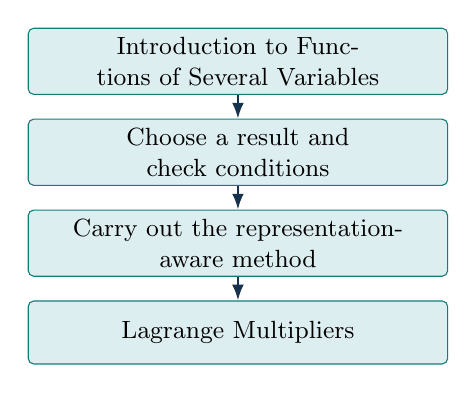
\begin{tikzpicture}[node distance=3mm, every node/.style={font=\small,align=center}, box/.style={draw=Teal,rounded corners=2pt,fill=Sky,minimum height=8mm,text width=0.42\textwidth}, arr/.style={-{Latex[length=2mm]},thick,draw=Ink}]
\node[box] (a) {Introduction to Functions of Several Variables};
\node[box,below=of a] (b) {Choose a result and check conditions};
\node[box,below=of b] (c) {Carry out the representation-aware method};
\node[box,below=of c] (d) {Lagrange Multipliers};
\draw[arr] (a)--(b); \draw[arr] (b)--(c); \draw[arr] (c)--(d);
\end{tikzpicture}
\end{center}
\end{minipage}

\section{Learning objectives}
\begin{enumerate}
\item Explain the central objects and hypotheses in 13.1 and 13.10.
\item Translate among algebraic, graphical, numerical, and verbal representations.
\item Select an appropriate formula or theorem before beginning symbolic work.
\item Carry out multi-step calculations while preserving domain, sign, orientation, and units.
\item Diagnose common errors by testing assumptions and checking the result independently.
\item Synthesize the chapter's methods into a reusable problem-solving workflow.
\end{enumerate}

\section{13.1 Introduction to Functions of Several Variables}
\begin{longtable}{C N}\cornellcuehead
\cornellcuerow{What is the governing idea in 13.1?}{A multivariable function maps points in a planar or spatial domain to values visualized by surfaces or level sets.}
\cornellcuerow{Which result should be recalled?}{\formula{z=f(x,y),\qquad f(x,y)=c\text{ defines a level curve}}}
\cornellcuerow{How should a problem be organized?}{Determine the domain, inspect traces and level sets, and connect units of inputs and output to the surface interpretation.}
\cornellcuerow{What should be checked before accepting an answer?}{Confirm the hypotheses and domain, preserve units and orientation when relevant, and substitute or differentiate back into the defining relation.}
\end{longtable}
\begin{warningbox}A two-dimensional contour plot omits height unless level labels and spacing are read carefully.\end{warningbox}
\begin{sectionsummarybox}A multivariable function maps points in a planar or spatial domain to values visualized by surfaces or level sets. The operational habit is to determine the domain, inspect traces and level sets, and connect units of inputs and output to the surface interpretation.\end{sectionsummarybox}
\section{13.2 Limits and Continuity}
\begin{longtable}{C N}\cornellcuehead
\cornellcuerow{What is the governing idea in 13.2?}{A multivariable limit must agree along every path toward a point; continuity combines that limit with the function value.}
\cornellcuerow{Which result should be recalled?}{\formula{\lim_{(x,y)\to(a,b)}f(x,y)=L}}
\cornellcuerow{How should a problem be organized?}{Try direct continuity first, use bounding or polar distance for proofs, and use two conflicting paths to disprove a limit.}
\cornellcuerow{What should be checked before accepting an answer?}{Confirm the hypotheses and domain, preserve units and orientation when relevant, and substitute or differentiate back into the defining relation.}
\end{longtable}
\begin{warningbox}Agreement along several chosen paths cannot by itself prove a multivariable limit exists.\end{warningbox}
\begin{sectionsummarybox}A multivariable limit must agree along every path toward a point; continuity combines that limit with the function value. The operational habit is to try direct continuity first, use bounding or polar distance for proofs, and use two conflicting paths to disprove a limit.\end{sectionsummarybox}
\section{13.3 Partial Derivatives}
\begin{longtable}{C N}\cornellcuehead
\cornellcuerow{What is the governing idea in 13.3?}{A partial derivative changes one input while holding the others fixed and provides coordinate-direction rates.}
\cornellcuerow{Which result should be recalled?}{\formula{f_x=\frac{\partial f}{\partial x},\qquad f_{xy}=\frac{\partial}{\partial y}(f_x)}}
\cornellcuerow{How should a problem be organized?}{Freeze nonactive variables, differentiate, evaluate at the requested point, and keep mixed-derivative order explicit.}
\cornellcuerow{What should be checked before accepting an answer?}{Confirm the hypotheses and domain, preserve units and orientation when relevant, and substitute or differentiate back into the defining relation.}
\end{longtable}
\begin{warningbox}Treating all variables as changing turns a partial derivative into a different calculation.\end{warningbox}
\begin{sectionsummarybox}A partial derivative changes one input while holding the others fixed and provides coordinate-direction rates. The operational habit is to freeze nonactive variables, differentiate, evaluate at the requested point, and keep mixed-derivative order explicit.\end{sectionsummarybox}
\section{13.4 Differentials}
\begin{longtable}{C N}\cornellcuehead
\cornellcuerow{What is the governing idea in 13.4?}{The total differential is the linear part of a small multivariable output change and supports error propagation.}
\cornellcuerow{Which result should be recalled?}{\formula{dz=f_x\,dx+f_y\,dy}}
\cornellcuerow{How should a problem be organized?}{Evaluate partial derivatives at the base point, multiply by signed input changes, and compare the estimate with exact change when available.}
\cornellcuerow{What should be checked before accepting an answer?}{Confirm the hypotheses and domain, preserve units and orientation when relevant, and substitute or differentiate back into the defining relation.}
\end{longtable}
\begin{warningbox}Adding absolute input errors with their original signs can understate a worst-case error bound.\end{warningbox}
\begin{sectionsummarybox}The total differential is the linear part of a small multivariable output change and supports error propagation. The operational habit is to evaluate partial derivatives at the base point, multiply by signed input changes, and compare the estimate with exact change when available.\end{sectionsummarybox}
\section{13.5 Chain Rules for Functions of Several Variables}
\begin{longtable}{C N}\cornellcuehead
\cornellcuerow{What is the governing idea in 13.5?}{Multivariable Chain Rules sum contributions along every dependency path.}
\cornellcuerow{Which result should be recalled?}{\formula{\frac{dz}{dt}=f_x\frac{dx}{dt}+f_y\frac{dy}{dt}}}
\cornellcuerow{How should a problem be organized?}{Draw a dependency tree, compute each local derivative, multiply along paths, and sum paths ending at the target variable.}
\cornellcuerow{What should be checked before accepting an answer?}{Confirm the hypotheses and domain, preserve units and orientation when relevant, and substitute or differentiate back into the defining relation.}
\end{longtable}
\begin{warningbox}Missing one dependency path omits part of the total rate.\end{warningbox}
\begin{sectionsummarybox}Multivariable Chain Rules sum contributions along every dependency path. The operational habit is to draw a dependency tree, compute each local derivative, multiply along paths, and sum paths ending at the target variable.\end{sectionsummarybox}
\section{13.6 Directional Derivatives and Gradients}
\begin{longtable}{C N}\cornellcuehead
\cornellcuerow{What is the governing idea in 13.6?}{The gradient points in the direction of steepest increase, and its dot product with a unit direction gives the directional derivative.}
\cornellcuerow{Which result should be recalled?}{\formula{D_{\mathbf u}f=\nabla f\cdot\mathbf u,\qquad \|\mathbf u\|=1}}
\cornellcuerow{How should a problem be organized?}{Compute the gradient at the point, normalize the requested direction, take the dot product, and interpret sign and magnitude.}
\cornellcuerow{What should be checked before accepting an answer?}{Confirm the hypotheses and domain, preserve units and orientation when relevant, and substitute or differentiate back into the defining relation.}
\end{longtable}
\begin{warningbox}Using a nonunit direction scales the result and no longer gives change per unit distance.\end{warningbox}
\begin{sectionsummarybox}The gradient points in the direction of steepest increase, and its dot product with a unit direction gives the directional derivative. The operational habit is to compute the gradient at the point, normalize the requested direction, take the dot product, and interpret sign and magnitude.\end{sectionsummarybox}
\section{13.7 Tangent Planes and Normal Lines}
\begin{longtable}{C N}\cornellcuehead
\cornellcuerow{What is the governing idea in 13.7?}{For a regular level surface, the gradient is normal and generates tangent-plane and normal-line equations.}
\cornellcuerow{Which result should be recalled?}{\formula{\nabla F(a,b,c)\cdot\langle x-a,y-b,z-c\rangle=0}}
\cornellcuerow{How should a problem be organized?}{Express the surface as $F=0$, evaluate a nonzero gradient, and use it consistently as the normal vector.}
\cornellcuerow{What should be checked before accepting an answer?}{Confirm the hypotheses and domain, preserve units and orientation when relevant, and substitute or differentiate back into the defining relation.}
\end{longtable}
\begin{warningbox}If the gradient vanishes, the standard tangent-plane formula provides no valid normal.\end{warningbox}
\begin{sectionsummarybox}For a regular level surface, the gradient is normal and generates tangent-plane and normal-line equations. The operational habit is to express the surface as $F=0$, evaluate a nonzero gradient, and use it consistently as the normal vector.\end{sectionsummarybox}
\section{13.8 Extrema of Functions of Two Variables}
\begin{longtable}{C N}\cornellcuehead
\cornellcuerow{What is the governing idea in 13.8?}{Interior local extrema occur at critical points, which the second-derivative test may classify.}
\cornellcuerow{Which result should be recalled?}{\formula{D=f_{xx}f_{yy}-f_{xy}^2}}
\cornellcuerow{How should a problem be organized?}{Find points where both first partials vanish or fail, compute $D$, apply the test, and analyze inconclusive cases separately.}
\cornellcuerow{What should be checked before accepting an answer?}{Confirm the hypotheses and domain, preserve units and orientation when relevant, and substitute or differentiate back into the defining relation.}
\end{longtable}
\begin{warningbox}$D=0$ is inconclusive rather than evidence of no extremum.\end{warningbox}
\begin{sectionsummarybox}Interior local extrema occur at critical points, which the second-derivative test may classify. The operational habit is to find points where both first partials vanish or fail, compute $D$, apply the test, and analyze inconclusive cases separately.\end{sectionsummarybox}
\section{13.9 Applications of Extrema}
\begin{longtable}{C N}\cornellcuehead
\cornellcuerow{What is the governing idea in 13.9?}{Applied multivariable optimization combines an objective, a feasible region, and interior and boundary candidates.}
\cornellcuerow{Which result should be recalled?}{\formula{\text{compare }f\text{ on interior critical points and the boundary}}}
\cornellcuerow{How should a problem be organized?}{Model the objective with units, determine whether the feasible set is closed and bounded, parameterize each boundary, and compare values.}
\cornellcuerow{What should be checked before accepting an answer?}{Confirm the hypotheses and domain, preserve units and orientation when relevant, and substitute or differentiate back into the defining relation.}
\end{longtable}
\begin{warningbox}Ignoring corners or boundary curves can miss an absolute optimum.\end{warningbox}
\begin{sectionsummarybox}Applied multivariable optimization combines an objective, a feasible region, and interior and boundary candidates. The operational habit is to model the objective with units, determine whether the feasible set is closed and bounded, parameterize each boundary, and compare values.\end{sectionsummarybox}
\section{13.10 Lagrange Multipliers}
\begin{longtable}{C N}\cornellcuehead
\cornellcuerow{What is the governing idea in 13.10?}{At a regular constrained extremum, objective and constraint gradients are parallel.}
\cornellcuerow{Which result should be recalled?}{\formula{\nabla f=\lambda\nabla g,\qquad g=c}}
\cornellcuerow{How should a problem be organized?}{Write all multiplier equations plus the constraint, solve every branch, reject infeasible points, and compare objective values.}
\cornellcuerow{What should be checked before accepting an answer?}{Confirm the hypotheses and domain, preserve units and orientation when relevant, and substitute or differentiate back into the defining relation.}
\end{longtable}
\begin{warningbox}The method needs regularity and does not replace checking singular constraint points or endpoints.\end{warningbox}
\begin{sectionsummarybox}At a regular constrained extremum, objective and constraint gradients are parallel. The operational habit is to write all multiplier equations plus the constraint, solve every branch, reject infeasible points, and compare objective values.\end{sectionsummarybox}

\section{Definitions and theorem register}
\small
\begin{longtable}{@{}>{\RaggedRight\arraybackslash}p{0.24\textwidth}>{\RaggedRight\arraybackslash}p{0.40\textwidth}>{\RaggedRight\arraybackslash}p{0.29\textwidth}@{}}
\toprule
\textbf{Topic} & \textbf{Meaning and conditions} & \textbf{Canonical form}\\
\midrule\endhead
13.1 Introduction to Functions of Several Variables & A multivariable function maps points in a planar or spatial domain to values visualized by surfaces or level sets. & \adjustbox{max width=\linewidth}{\(\displaystyle z=f(x,y),\qquad f(x,y)=c\text{ defines a level curve}\)} \\\addlinespace[2pt]
13.2 Limits and Continuity & A multivariable limit must agree along every path toward a point; continuity combines that limit with the function value. & \adjustbox{max width=\linewidth}{\(\displaystyle \lim_{(x,y)\to(a,b)}f(x,y)=L\)} \\\addlinespace[2pt]
13.3 Partial Derivatives & A partial derivative changes one input while holding the others fixed and provides coordinate-direction rates. & \adjustbox{max width=\linewidth}{\(\displaystyle f_x=\frac{\partial f}{\partial x},\qquad f_{xy}=\frac{\partial}{\partial y}(f_x)\)} \\\addlinespace[2pt]
13.4 Differentials & The total differential is the linear part of a small multivariable output change and supports error propagation. & \adjustbox{max width=\linewidth}{\(\displaystyle dz=f_x\,dx+f_y\,dy\)} \\\addlinespace[2pt]
13.5 Chain Rules for Functions of Several Variables & Multivariable Chain Rules sum contributions along every dependency path. & \adjustbox{max width=\linewidth}{\(\displaystyle \frac{dz}{dt}=f_x\frac{dx}{dt}+f_y\frac{dy}{dt}\)} \\\addlinespace[2pt]
13.6 Directional Derivatives and Gradients & The gradient points in the direction of steepest increase, and its dot product with a unit direction gives the directional derivative. & \adjustbox{max width=\linewidth}{\(\displaystyle D_{\mathbf u}f=\nabla f\cdot\mathbf u,\qquad \|\mathbf u\|=1\)} \\\addlinespace[2pt]
13.7 Tangent Planes and Normal Lines & For a regular level surface, the gradient is normal and generates tangent-plane and normal-line equations. & \adjustbox{max width=\linewidth}{\(\displaystyle \nabla F(a,b,c)\cdot\langle x-a,y-b,z-c\rangle=0\)} \\\addlinespace[2pt]
13.8 Extrema of Functions of Two Variables & Interior local extrema occur at critical points, which the second-derivative test may classify. & \adjustbox{max width=\linewidth}{\(\displaystyle D=f_{xx}f_{yy}-f_{xy}^2\)} \\\addlinespace[2pt]
13.9 Applications of Extrema & Applied multivariable optimization combines an objective, a feasible region, and interior and boundary candidates. & \adjustbox{max width=\linewidth}{\(\displaystyle \text{compare }f\text{ on interior critical points and the boundary}\)} \\\addlinespace[2pt]
13.10 Lagrange Multipliers & At a regular constrained extremum, objective and constraint gradients are parallel. & \adjustbox{max width=\linewidth}{\(\displaystyle \nabla f=\lambda\nabla g,\qquad g=c\)} \\\addlinespace[2pt]
\bottomrule
\end{longtable}
\normalsize

\section{Formula and method sheet}
\small
\begin{longtable}{@{}>{\RaggedRight\arraybackslash}p{0.08\textwidth}>{\RaggedRight\arraybackslash}p{0.48\textwidth}>{\RaggedRight\arraybackslash}p{0.37\textwidth}@{}}
\toprule
\textbf{Sec.} & \textbf{Method sequence} & \textbf{Stop-and-check trigger}\\
\midrule\endhead
13.1 & Determine the domain, inspect traces and level sets, and connect units of inputs and output to the surface interpretation. & A two-dimensional contour plot omits height unless level labels and spacing are read carefully. \\\addlinespace[2pt]
13.2 & Try direct continuity first, use bounding or polar distance for proofs, and use two conflicting paths to disprove a limit. & Agreement along several chosen paths cannot by itself prove a multivariable limit exists. \\\addlinespace[2pt]
13.3 & Freeze nonactive variables, differentiate, evaluate at the requested point, and keep mixed-derivative order explicit. & Treating all variables as changing turns a partial derivative into a different calculation. \\\addlinespace[2pt]
13.4 & Evaluate partial derivatives at the base point, multiply by signed input changes, and compare the estimate with exact change when available. & Adding absolute input errors with their original signs can understate a worst-case error bound. \\\addlinespace[2pt]
13.5 & Draw a dependency tree, compute each local derivative, multiply along paths, and sum paths ending at the target variable. & Missing one dependency path omits part of the total rate. \\\addlinespace[2pt]
13.6 & Compute the gradient at the point, normalize the requested direction, take the dot product, and interpret sign and magnitude. & Using a nonunit direction scales the result and no longer gives change per unit distance. \\\addlinespace[2pt]
13.7 & Express the surface as $F=0$, evaluate a nonzero gradient, and use it consistently as the normal vector. & If the gradient vanishes, the standard tangent-plane formula provides no valid normal. \\\addlinespace[2pt]
13.8 & Find points where both first partials vanish or fail, compute $D$, apply the test, and analyze inconclusive cases separately. & $D=0$ is inconclusive rather than evidence of no extremum. \\\addlinespace[2pt]
13.9 & Model the objective with units, determine whether the feasible set is closed and bounded, parameterize each boundary, and compare values. & Ignoring corners or boundary curves can miss an absolute optimum. \\\addlinespace[2pt]
13.10 & Write all multiplier equations plus the constraint, solve every branch, reject infeasible points, and compare objective values. & The method needs regularity and does not replace checking singular constraint points or endpoints. \\\addlinespace[2pt]
\bottomrule
\end{longtable}
\normalsize

\section{Common errors and diagnostic checks}
\begin{warningbox}
\begin{itemize}
\item \textbf{13.1:} A two-dimensional contour plot omits height unless level labels and spacing are read carefully.
\item \textbf{13.2:} Agreement along several chosen paths cannot by itself prove a multivariable limit exists.
\item \textbf{13.3:} Treating all variables as changing turns a partial derivative into a different calculation.
\item \textbf{13.4:} Adding absolute input errors with their original signs can understate a worst-case error bound.
\item \textbf{13.5:} Missing one dependency path omits part of the total rate.
\item \textbf{13.6:} Using a nonunit direction scales the result and no longer gives change per unit distance.
\item \textbf{13.7:} If the gradient vanishes, the standard tangent-plane formula provides no valid normal.
\item \textbf{13.8:} $D=0$ is inconclusive rather than evidence of no extremum.
\item \textbf{13.9:} Ignoring corners or boundary curves can miss an absolute optimum.
\item \textbf{13.10:} The method needs regularity and does not replace checking singular constraint points or endpoints.
\end{itemize}
\end{warningbox}
\begin{checkbox}
Before accepting any result: state the relevant domain; check theorem hypotheses; estimate sign and scale; preserve units and orientation; and verify by substitution, differentiation, a limiting case, or a second representation.
\end{checkbox}

\section{Chapter synthesis}
Extend limits, derivatives, approximation, optimization, and constraints from one input to several interacting variables. The chapter begins with \textbf{Introduction to Functions of Several Variables} and culminates in \textbf{Lagrange Multipliers}. Across the sequence, the most reliable workflow is to identify the mathematical object, choose a representation, state the governing result with its hypotheses, compute without dropping restrictions, and audit the answer against the original definition. Multivariable calculus is organized by local linear structure: paths test limits, gradients encode first-order change, and feasible-set geometry governs optimization.

\section{Self-test questions}
\begin{enumerate}
\item Explain the central distinction or object in 13.1, using both words and notation.
\item State the main formula or result from 13.2 and identify every hypothesis or restriction needed for its use.
\item Describe the problem-solving procedure for 13.3. What is the strongest independent check?
\item Compare the roles of Introduction to Functions of Several Variables and Lagrange Multipliers within this chapter.
\item Reconstruct the governing formula for 13.4 from its geometric or analytic meaning.
\item Choose one method in the chapter and explain how its output should be interpreted, including units or orientation when applicable.
\item Scenario: A student working on 13.1 produces a polished calculation but makes this error: A two-dimensional contour plot omits height unless level labels and spacing are read carefully. Diagnose the earliest invalid step and repair the workflow.
\item Scenario: A solution in 13.2 quotes the displayed formula without checking conditions. Which conditions must be checked, and what could fail if they are absent?
\item Construct a concept map linking a representation, a governing result, a computation, and a verification check from this chapter.
\item Design a two-part test for mastery: one conceptual prompt and one calculation. State what evidence would count as a complete answer.
\end{enumerate}

\Needspace{8\baselineskip}
\section{Answer key}
\small
\begin{enumerate}
\item A complete response identifies A multivariable function maps points in a planar or spatial domain to values visualized by surfaces or level sets. It should connect that meaning to \(z=f(x,y),\qquad f(x,y)=c\text{ defines a level curve}\) and state the relevant domain.
\item The organizing result is \(\lim_{(x,y)\to(a,b)}f(x,y)=L\). The solver must check that the quantities are defined and that the assumptions named in 13.2 hold before applying it.
\item Use this sequence: Freeze nonactive variables, differentiate, evaluate at the requested point, and keep mixed-derivative order explicit. The strongest check is to return to the defining relation or differentiate/substitute the result, as appropriate.
\item Introduction to Functions of Several Variables establishes a multivariable function maps points in a planar or spatial domain to values visualized by surfaces or level sets. Lagrange Multipliers extends the chapter to at a regular constrained extremum, objective and constraint gradients are parallel. The connection is the reuse of the same representations under a broader method.
\item The formula \(dz=f_x\,dx+f_y\,dy\) follows by translating the defining geometric or rate relationship into symbols; each factor records a distinct change or scale.
\item Interpretation must name what varies, with respect to what, and on which domain. A numerical value without units, sign, direction, or interval information is incomplete whenever those features are part of the modeled quantity.
\item The earliest fault is the unverified assumption described by this warning: A two-dimensional contour plot omits height unless level labels and spacing are read carefully. Restart by following this procedure: Determine the domain, inspect traces and level sets, and connect units of inputs and output to the surface interpretation.
\item The formula \(\lim_{(x,y)\to(a,b)}f(x,y)=L\) is conditional, not decorative. Check domain, differentiability or integrability as relevant, boundary or orientation requirements, and nonzero denominators before drawing a conclusion.
\item One valid map is: the representation in 13.1 identifies the object; the result in 13.2 supplies a rule; the method in 13.3 carries out the computation; the check in 13.10 tests the conclusion against its definition.
\item The conceptual prompt should require explanation of a definition and its hypotheses. The calculation should require method selection rather than direct substitution. Full evidence includes setup, justified transformations, a result, and an independent check.
\end{enumerate}
\normalsize

\section{Key-term recap}
\small
\begin{longtable}{@{}>{\RaggedRight\arraybackslash}p{0.29\textwidth}>{\RaggedRight\arraybackslash}p{0.64\textwidth}@{}}
\toprule
\textbf{Term} & \textbf{Working meaning}\\
\midrule\endhead
Introduction to Functions of Several Variables & A multivariable function maps points in a planar or spatial domain to values visualized by surfaces or level sets. \\\addlinespace[2pt]
Limits and Continuity & A multivariable limit must agree along every path toward a point; continuity combines that limit with the function value. \\\addlinespace[2pt]
Partial Derivatives & A partial derivative changes one input while holding the others fixed and provides coordinate-direction rates. \\\addlinespace[2pt]
Differentials & The total differential is the linear part of a small multivariable output change and supports error propagation. \\\addlinespace[2pt]
Chain Rules for Functions of Several Variables & Multivariable Chain Rules sum contributions along every dependency path. \\\addlinespace[2pt]
Directional Derivatives and Gradients & The gradient points in the direction of steepest increase, and its dot product with a unit direction gives the directional derivative. \\\addlinespace[2pt]
Tangent Planes and Normal Lines & For a regular level surface, the gradient is normal and generates tangent-plane and normal-line equations. \\\addlinespace[2pt]
Extrema of Functions of Two Variables & Interior local extrema occur at critical points, which the second-derivative test may classify. \\\addlinespace[2pt]
Applications of Extrema & Applied multivariable optimization combines an objective, a feasible region, and interior and boundary candidates. \\\addlinespace[2pt]
Lagrange Multipliers & At a regular constrained extremum, objective and constraint gradients are parallel. \\\addlinespace[2pt]
\bottomrule
\end{longtable}
\normalsize

\enlargethispage{4\baselineskip}
\begin{tcolorbox}[title=One-sentence takeaway,fonttitle=\bfseries,colback=Ink,colframe=Ink,coltext=white,coltitle=white,arc=2mm,boxrule=0pt]
\centering\bfseries Multivariable calculus is organized by local linear structure: paths test limits, gradients encode first-order change, and feasible-set geometry governs optimization.
\end{tcolorbox}
\end{document}
